\documentclass{article}

\usepackage[dvipsnames]{xcolor}
\newcommand{\tom}[1]{{\textit{\color{WildStrawberry}{[#1]}}}}
\usepackage{graphicx}

\title{Meeting Updates}
\author{Joshua Fowler}

%\usepackage{Sweave}
\begin{document}
%\input{MeetingUpdates-concordance}
%\SweaveOpts{concordance=TRUE}
  \maketitle
  Tom's comments are in \tom{WildStrawberry}.

\section*{Josh's Spring 2020 Semester Work Plan}
\subsection*{Overall Goals}
\begin{itemize}
\item{Pass Qualifying exam with flying colors}
\item{Have mutualism range limits review paper in a submittable place by end of semester}
\item{Have climate explicit analysis of the stochastic demography project}
\item{Replace transplanted plants in range limit experiment}
\item{Restart Indiana Plots}
\item{Present on Herbarium project for Science Day and for ASN virtual conference in January}
\item{Apply for Sigma Xi, and ecolab funding, maybe others}
\end{itemize}

\subsection*{August}
\begin{itemize}
\item{Start moving seeds from growth chamber into GH if germinating}
\item{Work on quals proposal}
\item{Submit ASN abstract}
\end{itemize}
\subsection*{September}
\begin{itemize}
\item{Sept 1st: Have draft of Qualifying exam proposal}
\item{early Sept: Continue moving plants in to the greenhouse}
\item{mid Sept: Agronostics (need to order kits)}
\item{2 weeks before Quals: send proposal to committee}
\item{Sept 24 - Oct 10: Josh in Washington}
\item{Sept 24 - Oct 10: Finalize Quals presentation, submit Sigma Xi and Ecolab, and where possible work on revising Mutualism Range Limits}
\end{itemize}
\subsection*{October}
\begin{itemize}
\item{Oct 1: Sigma Xi grant due}
\item{Oct 4: Ecolab grant due}
\item{Qualifying exam in early Oct. Date TBD}
\item{Mid Oct: Depending on plant availability, restart Indiana plants}
\item{Late Oct - Early Nov: Visit Range limit sites to start AGHY plots and replace ELVI and POAU. Not sure if this will involve a seed experiment. I have definitely could do this with AGHY and POAU, but not with ELVI, and the POAU don't have E+ and E- lines}
\end{itemize}
\subsection*{November}
\begin{itemize}
\item{Depending on Ella and Lani's progress, would do some seed scoring of herbarium samples, and this past Summer's ecolab AGHY collections}
\item{Late Nov - Dec: Finalize Mutualism range limits review}
\end{itemize}
\subsection*{December}
\begin{itemize}
\item{Early Dec: Science Day}
\item{Work on Mutualism Range Limits review}
\item{Build climate explicit vital rate models}
\end{itemize}
\subsection*{January}
\begin{itemize}
\item{ASN conference Jan 9-11}
\end{itemize}



\section*{June 3, 2020}
\subsection*{Meeting Overview}
\textbf{We talked about:}
Some updates for the REU projects this Summer, the intro for the Stochastic demography manuscript as well as the figures/next steps for the project.

For next week (and Beyond):
\begin{itemize}
\item{Josh will follow up with BRIT and contact A+M about Summer sampling.}
\item{We will be meeting with Lani and Ella on Monday (time TBD)}
\item{Josh will look at what seed samples are remaining that need to be scored}
\item{Josh will look at Tom's comments on Intro}
\item{Josh will clean up the github repo}
\item{Josh will finish working on the data merging, and make sure that the workflow goes smoothly into the models}
\item{I'm not sure this will be done by next week, but Tom notes that we need to make sure that the models are actually fitting well}
\item{After checking model fitting, Josh will work on environmental correlations and forecasting.}
\item{We agreed we need the following figures: vital rate buffering (not sure what this figure looks like), contribution of variance to stochastic growth rate, environmental correlation (not sure what the story is), and something that does forecast, plus a figure that is all the vital rates in the supplement.}
\item{Josh is going to work on the mutualism range limits manuscript for next week. Hopefully, will have addressed the comments in introduction and added to the examples for each mechanism.}
\end{itemize}

\section*{May 27, 2020}
\subsection*{Meeting Overview}
\textbf{We talked about:}
Outline for the stochastic demography MS and some general updates for LTREB data processing, and for Summer REUs. 

Next week we will talk about:
\begin{itemize}
\item{Tom will read Stoch. Demo. Intro, and give feedback}
\item{We will sketch out what are the final figures for this paper}
\item{Josh will integrate 2020 data so far into the dropbox, and clean up the 2019 data merging}
\end{itemize}

\section*{May 20, 2020}
\subsection*{Meeting Overview}
\textbf{We talked about:}
Keeping up progress on the stochastic demography project, we have contacted new herbaria about the herbarium project and summer REU projects, virtual ESA meeting, and our upcoming meeting for the mutualism range limits project.
\begin{itemize}
\item{Meeting for Mutualism Range limits with Judie - May 25th}

Josh will work on the Tables and fleshing out text for the mechanisms with Marion

Tom will work on the box for the technical details of population analysis

\item{Stochastic Demography - We will be presenting a poster for this project at ESA. I think it would be great to be able to include final figures and climate projections into this. By the end of the summer, I'd like to have the manuscript in a submission ready place.}

*Tom has the plants that will be planted in Indiana, and is working on splitting them out

*For next week, Josh will have a draft of the introduction to discuss with Tom.

*Shaun and Mark are working on data collection at the plots already, and there is a possibility that some of us will go out in July as well to collect the rest of the plots.


*Josh will double check the TNF plants within the 2019 data, making sure that they are counted as dead, or to match up larger, new recruits to existing plants based on location.

*Josh will double check that the data processing script is including the 2019 data.

*In 2 weeks, for Jun 3rd. I have a tentative goal to have the data clean up settled, as this will help with writing the results and doing climate simulations.

*Other steps with less clear timelines:
\begin{itemize}
\item{writing methods (this is partially started)}
\item{simulations for climate change}
\item{plant traits, which was one of the topics discussed in the committee meeting}
\item{final figures (We need to consolidate the analysis to the full species models, which Tom has already worked on, but there is still some messiness in the code where we have both versions of the models)}
\item{writing results}
\item{writing discussion}
\end{itemize}

\item{ESA Virtual meeting - Aug 3-6th, (I'm not sure of the dates to submit the actual poster)}

\end{itemize}

  
\section*{April 1, 2020}
\subsection*{Meeting Overview}
\textbf{We talked about:}
Josh's upcoming committee meeting and how we will modify plans for field collections and experiments this summer given Covid19 travel restrictions. We decided that we won't set up the AGHY portion of the experiment this spring.
\begin{itemize}
\item{Mutualism Range Limits writing group with Marion: Thursday and Friday, the 2nd and 3rd.}
\item{Josh's committee meeting: Friday, Apr 10th (Josh will send a reminder on Monday and set up zoom on Thursday)}
\item{Make a decision about seed collection needs for this Summer by Wed. Apr. 15th. Josh or Tom will inventory seeds that we have in the fridge. The needs will depend on decisions related to experiments that we are going to set up (seed germination plots for current experiment, and/or an additional competition experiment.}
\item{We now have good starts on the Range Limits and the stochastic demography manuscripts. I'd like to schedule other dedicated time to work on these with a tentative goal of having the manuscripts written by the end of this Summer.}
\end{itemize}

  
\section*{Sep 24, 2019}
\subsection*{Meeting Overview}
\textbf{We talked about:}
 Primarily experimental design for the range limit project. We also talked about general seed updates and Josh's visit with Keith Clay.
 
 \subsection*{Notes:}
 Figure \ref{fig:rangelimitsexpdesign} shows a diagram of the proposed experimental design.
 \begin{figure}[h!]
 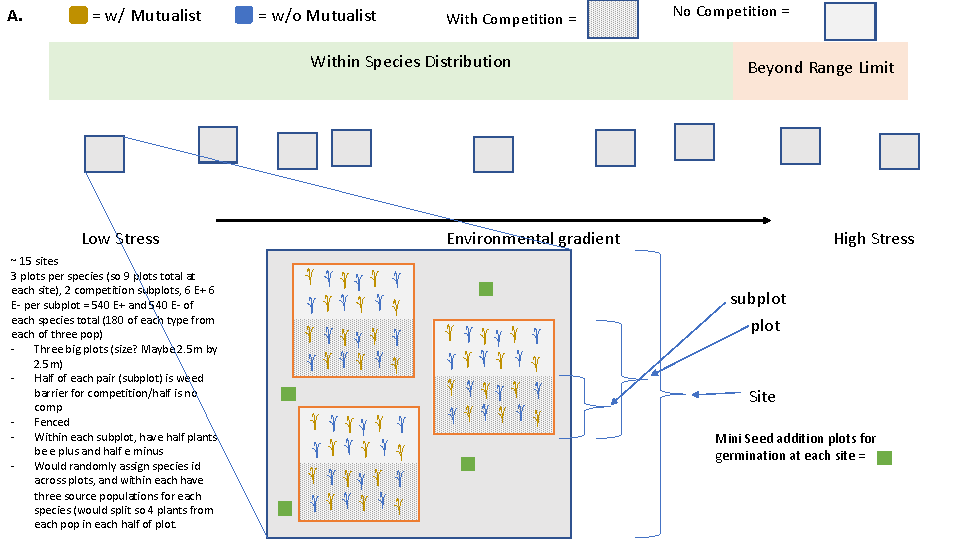
\includegraphics[width = \linewidth]{rangelimitsexpdesign.pdf}
 \caption{Proposed experimental design}
 \label{fig:rangelimitsexpdesign}
 \end{figure}
 \begin{itemize}
 \item{We are looking at approx. 15 sites across TX/LA/MS. I have contacted Bret Elderd to get some addition feedback about locations and will reach out to others. I think next steps include reaching out more specifically to have a more definitive set of sites.}
 \item{At each site, the plan is to have 9 plots, with three plots of each species, with the species assigned randomly across plots.}
 \item{The plots will be something like 2.5 m2. Potentially rectangular to make install of weed barrier easier. They will have a competition treatment subplot that covers half the plot.}
 \item{The competition treatment will be a weed barrier. In both subplots, the area immediatly around the new transplants will be cleared, but the competition subplot will have the vegetation cut back and a weed barrier install. They make white weed barrier, although it is less common, generally in 3 or 4 ft width. Could plan to cover both subplots with a layer of straw to reduce heat sink in the weedbarrier.}
 \item{Within each subplot, they will have 6 E+ and 6 E- plants coming evenly from three populations or population clusters of the species.}
 \item{This means there will be 540 E+ and 540 E- total plants of each species required.}
 \end{itemize}
 
 
 \section*{Sep 17, 2019}
 \subsection*{Meeting Overview}
 \textbf{We talked about:}
 General updates for the plant generation, narrowing down experimental design for the transplant experiment, and some updates on the stochastic demography project. Josh is also going to send a draft of the GRFP to Tom for feedback for next week. 
 
 \subsection*{Notes:}
 \begin{itemize}
 \item{Field sites}
 
 - Josh shared google maps list of potential sites. Will continue to update this, and plan to contact sites once we have a design finalized.
 
 -General notes for picking sites:
 
 * Contact local universities about field locations. (LSU, Tulane, SFASU, etc.)
 
 * Avoid federal land due to permits, although a few sites would be okay.
 
 * Think about habitat requirements, i.e. partial shade. Need somewhat different setup for different species, but also don't necessarily need pristine natural park, can use semi-natural areas, especially for AGHY and ELVI. 
 
 \item{Experimental Design}
 
 - Josh will draw up proposed designs and we will talk about them next week. 
 
 
 \item{Stochastic demography}
 
 - Tom will update the 2019 data
 
 - Josh is working on the merge, which is mostly set up. Need to revise the spikelet data to include model for counts. Currently, have been calculating an average. 
 
 \item{Other stuff}
 
 - Lani is working on the herbarium project. Josh needs to get back in contact with Texas AM to get their database of plants. Also need to get undergrads to work on photo transcription.
 
 - Ecolab is due OCT. 4.
 
 \end{itemize}
 
\section*{Aug 5, 2019}
\subsection*{Meeting Overview}
\textbf{We talked about:}
Catching up with stochastic demography progress and new data, and about the timeline for the Range limit experiment.

\subsection*{Notes:}
\begin{itemize}
\item{\textbf{Stochastic demography stuff}
\textbf{2019 data updates and pipeline for integration}

-   Tom will update 2019 field data with Elmyus spp and LOAR repro data

-   Tom will follow up with Jenn and Shaun about whether they were recording seeds or spikelets in Elymus

\textbf{Model questions and data issues}

-   Josh has a bunch of data merge and manipulation steps, but no major problems that we foresee

-   Unclear how often seedlings exceed seeds form prev year. Josh will update with latest data merges and see if we need to account for seed bank (hopefully not)

-   Josh will merge into individual level endophyte scores and check with Jenn about questions that arise and apply these forward and backward in time (was there every a doubly scored plant and did it ever change?)

-   Josh will also merge in distance data beginning in 2018 and apply these forward and backward in time
Next steps for population model and climate covariates

-   Goal: 6 time-varying vital rate models for E+ and E- of each species: survival, growth, flowering prob, inflorescence production of flowering plants, spikelets per inf, recruitment probability--**this is a good point to pass off results to Tom in late Sept / early Oct

-   Check with Jenn about climate data from Nashville and check the climate data files that she already provided}

\item{\textbf{Range limits experiment:}
\textbf{Plant rearing}

-   Tom will ask Jessica to clean out greenhouse (and will cc Josh) and wash pots

-   We will share a table of all the populations; these will move into the disinfection workflow: (1) apply heat (or control), (2) surface sterilize, (3) transfer to agar plate (need to be well sealed), (4) bring to cold room ~4-6 weeks, (5) growth change, (6) greenhouse, (7) arginostics

\textbf{Sites}
-   Alexandria-to-Junction swath—need to nail down specific sites. Sites that we already have some knowledge of are: Junction, Pontotoc (double helix ranch), Bastrop, Huntsville, Alexandria.

\textbf{Experimental design}

-   We need an experimental design – Josh will draft a few options (will the plots be fenced?)}

\end{itemize}


\subsection*{Goals and Timeline}
\begin{itemize}

\item{mid to end of Aug. - Heat treatments of seeds}
\item{mid to end of Aug. - Josh draws up experimental designs options.} 
\item{end of Aug.- Start germination for already treated seeds (AGHY and ELVI)}
\item{end of Aug. to mid Sept. - surface sterilize and start cold stratification (4-6 weeks)}
\item{end of Sept. or early Oct. - start seeds in growth chamber. (2-4 weeks)}
\item{end of Sept. or early Oct. - Email potential field sites. finalize experimental design.}
\item{Oct - November - potentially visit sites to scout locations, and pilot of competition treatment}
\item{end of Sept. or early Oct. - Goal to have all the vital rate models together to work with Tom on the population model.}
\item{Oct. 21 - NSF GRFP due.}
\item{Oct or November - potentially visit sites to scout locations, and pilot of competition treatment}

\item{end of Oct. or early Nov. transplant germinants to soil.}
\item{Late Nov. or Dec. Score plants with Agronostics.}
\item{Dec or Jan. or Feb. set up sites and tranplant plants into the field experiment.}
\end{itemize}
 
  
  
\section*{Apr 17, 2019}
\subsection*{Meeting Overview}
\textbf{We talked about:}
The early Summer Fieldwork schedule, and plans for visiting herbaria. We also talked about continuing issues with the fertility models. 

\subsection*{Updates on Goals from last meeting:}
\begin{itemize}
\item{\textbf{Range limit project:} I have a growing database with collection information, and we laid out a general schedule for fieldwork for the Summer. I need to come up with more specific plans for collection locations near our various other field trips. This also includes having a map of the Ecolab sites to be able to look for collections nearby.
Overall, the schedule includes:
\begin{itemize}
\item{April 20-21 - Local collections  - Josh}
\item{April 25-26 - Nagadoches Fieldwork - Tom, Josh, Kyle?}
\item{May 1-3 - Ecolab sites - Tom, Josh, Kyle}
\item{May 6-? Eastern collections trip - Josh}
\item{May 17-19 - Josh in Tucson}
\item{May 20-30 - SEV trip}
\item{June 3-7 - Indiana trip}
\item{June 10-14 (exact dates TBD) - Josh in Seattle}
\item{July 22or29 - ? Indiana trip}
\end{itemize}
}
\item{\textbf{Herbarium project:} For the Herbarium project, I have recommendations of herbaria with major grass collections from Bob Shaw, but this requires follow up with the actual herbaria. In general, we kind of talked about focusing on the major Texas herbaria, especially to start. Possibly planning this for June 7-10ish}
\item{\textbf{Stochastic demography:} I updated the flowering and fertility models to include data from the same year t, but I haven't rerun the flowering model and saved the outputs. I rewrote the seed to seedling model as a binomial, but this has a constriction that the number of seeds must be greater than the number of recruits. We talked about solutions for this today, and this also relates using Jenn's seed data, which I have been doing mostly to start simpler. Basically we decided that we want to move forward with the other seed means data first, so that we know how much this is a problem for our actual data. The convergence problems with the negative binomial model are likely not related to the function that I am using, but we talked about simplifying the model and seeing if the problems persist.}
\end{itemize}

\subsection*{Goals for Next meeting (Tom will be gone on the 24th, but I will email updates):}
\begin{itemize}
\item{\textbf{Range limit project:} I will map our Ecolab sites. From that I will have a database of nearby collection location possibilities to the ecolab sites and to the Nagadoches trip. I plan to do some local collection this weekend.}
\item{\textbf{Herbarium project:} I will contact the herbaria on my list to get more info about their collections. This will also be a necessary first step of setting up actual premission and times to sample at the herbaria. Generally we plan on starting with the Texas herbaria, and holding off on this until after collecting seeds from the field during peak seed time for early flowering species.}
\item{\textbf{Stochastic demography:} I will do the fertility model debugging by looking at models of the mean and building up. I will also finish the seed models that I have been working on to have seed data to work with within the seed to seedling transition model. Then I will be able to table where we actually have more seedlings than seeds. I will also finish the Readme file and clean up the project folder a bit to keep notes for where I am in the project. I also have a goal to move the figures into Rmarkdown.}
\end{itemize}
 
 
\section*{Apr 10, 2019}
\subsection*{Meeting Overview}
\textbf{We talked about:}
Field work scheduling stuff, plant collection plans, and reproductive models!

\subsection*{Updates on Goals from last meeting:}
\begin{itemize}
\item{\textbf{Range limit project:} I have looked at collection data and have looked at general patterns, which I think point out some promising counties, which I can use to create a database with specific collection locations info. We also talked about collecting at least three populations of each species for the final experiment and about looking for opportunities for collections from near Ecolab sites and near Nagadoches. Tom also wants to collect Festuca paradoxa.}
\item{\textbf{Herbarium project:} I will be in contact with Bob Shaw at A\&M But I haven't generated an actual list of herbaria.}
\item{\textbf{Stochastic demography:} I have run the seed to seedling model, and seed means. There are several issues that we talked about that I will work on for next week, but overall it was productive. I didn't save the residual plots, but I have been working on that and will continue to do so for more of the models.}
\end{itemize}

\subsection*{Goals for Next meeting:}
\begin{itemize}
\item{\textbf{Range limit project:} I would like to have a database of collection locations and  tentative travel calendar for next week.}
\item{\textbf{Herbarium project:} I will hopefully have a list of the best herbaria to visit, and include these visits in the calendar}
\item{\textbf{Stochastic demography:} I will update the things we talked about in the models: Looking into the link function for the fertility model (and the other negative binomial models), updating the seed to seedling model to a binomial model, and adding an organizational document to track progress within the project.}
\end{itemize}
 

\section*{Apr 3, 2019}
\subsection*{Meeting Overview}
\textbf{We talked about:}
\begin{itemize}
\item{Trends in endophyte prevalence from the Sneck and the Rudgers data. Based on our meeting, I altered the plots to show just Longitude trends, and incorporated ecolab data. Overall, I narrowed to a list of 5-6 interesting species, Poa autumnalis, Elymus virginicus, Agrostis hyemalis, Agrostis perennans, and Sphenopholis nitida, and possibly Elymus canadensis}
\item{We didn't talk too much about the stochastic demography stuff, but that is my major goal for next week.}
\end{itemize}

\subsection*{Updates on Goals from last meeting:}
\begin{itemize}
\item{\textbf{Range limit project:} I have gotten a pretty good list of candidate species for the project and we are generally converged on the idea of a Southeast transect of species. There are interesting trends in some of the species, and generally there is variability in infection prevalence even in the highly infected species, which I think are good signs that there could be context dependence in the interaction (although probably to varying degrees).}
\item{\textbf{Herbarium project:} We didn't have a huge update from this project. I submitted the Native plant society grant last week related to this project.}
\item{\textbf{Stochastic demography:} We talked about this briefly, but overall, I have started working on the seed-to-seedling model and have looked at the fertility data generally, but I need to do so in a more systematic way. I also need to finish the PPC's for the models. This is my main goal for next week's meeting. We also talked about making sure that I have documentation for all of my progress as we go into the busy summer fieldwork season.}
\end{itemize}

\subsection*{Goals for Next meeting:}
\begin{itemize}
\item{\textbf{Range limit project:} I am going to make a seed collection schedule for the coming months and early Summer. For next week, I will look at herbarium records for the species we are considering and get some general phenology info across the range that I can use to plan collecting trips. I will start with that and start a database to keep track of what is currently available and possible collection locations.}
\item{\textbf{Herbarium project:} For this project, we talked about how there is less pressing collection needs, but I think that Tom's suggestion of contacting the A\&M herbarium would be a good place to start to find the main grass herbaria. Longer term, I want to have a list of herbaria that I plan to visit over the Summer.}
\item{\textbf{Stochastic demography:} My main goals for next week are focused on the stochastic demography project. I will update on the fertility data issues, I'd like to have residual plots for all of the models run so far, and I want to have run the seed to seedling model for next week.}
\end{itemize}


\section*{Mar 29, 2019}
\subsection*{Meeting Overview}
\textbf{We talked about:}
\begin{itemize}
\item{Figures from growth, survival, and flowering models. We also discussed the fertility model issues,and credible intervals.}
\item{Follow up from feedback from the committee meeting primarily about the range limit project and the herbarium work.}
\end{itemize}

\subsection*{Updates on Goals from Committee meeting and earlier}
\begin{itemize}
\item{I have run the fertility model, but there are issues with certain species and I need to double check that I am correctly splitting up the data.}
\item{We talked about upcoming field work and some of the main points from the committee feedback. In general, we are mostly set on doing a Southeastern continental gradient.}
\item{In general, I will continue to develop the conceptual background for the projects. I want to set a goal of adding 5 papers per week to the annotated bibliographies for the range limits and the herbarium projects.}
\end{itemize}

\subsection*{Goals for next week}
\begin{itemize}
\item{\textbf{For the Range limit project:} Explore Jenn's endophyte database and look for species with trends in endophyte prevalence. Ideally, we will have a mostly set idea of species with which we want to work.}
\item{\textbf{For the Stochastic demography project:} I will work on posterior predictive checks for the models. I will also make sure that my fertility model is using the correct data, and if it is, I will table up the data to look at where it is actually a problem. I will also update my dropbox so that I can share the model runs with Tom. I most likely won't get it done by Wednesday, but other goals include the seed-to-seedling model, and the models for seed production.}
\end{itemize}

\section*{Mar 6, 2019}
\subsection*{Meeting Overview}
\textbf{We talked about:}
\begin{itemize}
\item{Looked at start of my figure from survival and flowering models}
\item{Talked about sites for the Range limit project and identified some outstanding questions and things to think about to plan this.}
\end{itemize}

\subsection*{Update on goals from last week}
\begin{itemize}
\item{I have results from the flowering and survival models rerun. I need to finish running the growth models.}
\item{I looked at field stations and have the idea of doing a northern and a southern transect. We had a good discussion about this, and I will keep looking into these.}
\item{For the Herbarium project, I have continued to read and add to my annotated bib., but I need to look more specifically for our target species.}
\end{itemize}

\subsection*{Goals for next meeting:}
\begin{itemize}
\item{\textbf{Stochastic demography:}Finish running the growth models. Have a figure by friday. Systematically check model diagnostics for the models runs by next week. Write up code for Fertility (NegBinomial), and possibly run it. Quantify the sample size of each year of each species for the various reproductive measurements. On the horizon, we have the seed to seedling transition model, and then integrating these into the matrix model.}
\item{\textbf{Range limit project:} We had a good discussion about the transect replication, and what species are available. For Next week, a major goal, would be to have a GIS map with field stations and the species distributions. Otherwise, I want to think more about the pros and cons of the different replication schema that we discussed. Additionally, I will think about the competition treatment. I will continue to read, but also, I will try to alter our hypothesis figure including competition.}
\item{\textbf{Herbarium project:} Include in the annotated bibliography our range limit "focal" species. For next week, I'll have another look at the set of questions, and come up with a pros/cons list of the projects get feedback on at my committee meeting.}
\end{itemize}
  
  
\section*{Feb 27, 2019}
\subsection*{Meeting Overview}
\textbf{We talked about the challenges from last week.}

\subsection*{Update on goals from last week}
\begin{itemize}
\item{I did not have results from the stochastic demography models due to memory issues. We decided to go back to single species models.}
\item{We went over the annotated bibliography for the herbarium project. I feel that I am at ~75 percent coverage of the literature. I think that there are interesting trends in what people have found looking at the relationship between endophytes and environmental factors. No one seems to have look at endophytes over time specifically. We talked about defining our research questions for this project and whether this satisfies the types of info we would want for the range limit question, and whether the temporal aspect is worth doing, or if there is some other broader question that would appropriate to look at with herbaria.}
\item{For the range limit project, we talked about the second draft of research questions. I think this was productive, and will continue to refine these.}
\end{itemize}

\subsection*{Goals for next week:}
\begin{itemize}
\item{For the stochastic demography: going back to single species models have results from the surv, growth, and flowering models and make a "beautiful figure".}
\item{For the Herbarium project: Continue to add to the annotated bibliography. Look specifically for surveys and patterns for the three species we have been talking about for the range limit project. Also, look for symbioses beyond endophytes/fungi.}
\item{For the Range limit project: Choose prospective sites for the transects in the experiment. Also, unpack the research questions more into separate questions.}
\end{itemize}

\section*{Feb 18, 2019}
\subsection*{Meeting Overview}
\textbf{This meeting was shorter, but we established some goals for next week's meeting. We talked about:}
\begin{itemize}
\item{Stochastic demography results from survival, growth and flowering models}
\item{Annotated bibliography for the herbarium project}
\item{2nd draft of questions for the range limit question and for the herbarium project}
\end{itemize}

\section*{Feb 13, 2019}
\subsection*{Meeting Overview}
\textbf{We talked about:}
\begin{itemize}
\item{A progress update on the stochastic demography project}
\item{For the herbarium project, we talked about the eventual size of this project, and how that will be driven by our questions and predictions for environmental change.}
\item{For the range limit project, we talked about the research question and about a general experimental design.}
\end{itemize}

\subsection*{Update on Goals from last meeting:}
\begin{itemize}
\item{\textbf{Stochastic demography:} The data is mergeable, and I have a script laid out for the growth model, but it does not account for the zero-inflated negative binomial. I need to look at vectorization for the year random effect still, and I have not had a true run of the models as written with loops.}
\item{\textbf{Herbarium project:} I have seed and some tissue samples from Mercer gardens. We did some seed squashes and saw endophytes which is really cool.}
\item{\textbf{Range limit project:} We talked about the questions and experimental design. I will continue to work on these. We didn't talk about this a ton, but thinking about Spring and Summer fieldwork, it looks like I will want to collect plants from across the range, and potentially along multiple transects. We also briefly talked about getting a sense of the seeds that we have on hand already.}
\item{\textbf{Committee meeting:}I have heard back now from everyone, and will go ahead with scheduling.}
\end{itemize}

\subsection*{Goals for next meeting:}
\begin{itemize}
\item{\textbf{Stochastic demography:} Incorporate model vectorization for the flowering and survival models and/or figure out if that is just not worth it. Add mixture model for the zero truncated distribution in the growth model.}
\item{\textbf{Herbarium project:} Perform a mini endophyte id experiment with the seeds from Mercer. I will primarily compare the seed squash and the agronostics. There is also the "pithe scraping" method, which I'm not sure that we have good enough samples for, but I will try to figure out what that method entails. 
Another goal is to be familiar with the endophyte range survey literature, and any similar herbaria project literature. This will be an ongoing process, but I would like to have something started for next week. This will also aid in refining the questions here.}
\item{\textbf{Range limit project:} Thinking about the experimental design in actual geographic space, locate possible sites for common garden plots. Related to the work with PRISM for the LTER project, I will spend some time working with climate maps, which I haven't had a ton of experience with. 
Bring draft 2 of the research question, revise it to be more specific.}
\item{\textbf{Committee meeting:} I will schedule this officially, and contact Rachael about a room. I will also make an outline presentation for myself, which will be the landing site for the various research questions that I am refining across the projects.}
\end{itemize}


\section*{Feb 7, 2019}
\subsection*{Progress Update}
\begin{itemize}
\item{\textbf{Stochastic demography:}
I have good progress on the flowering and seed data script. Overall, there is flowering tiller information for everything, barring a few NAs from data entry. There is information about the spikelets/inflorescence for a subset of the plants, but this is actually measured, and not estimated. It depends on the plant, but some have one inflorescence measured and some have up to 3 measured. There is seeds/spikelet information for even less plants than for spikelets. In the raw data sheets, there is often seed info, but it is basically just multiplied number of spikelets by some average that was calculated based on the seeds/spikelet data. So the way I am currently pulling in the data is to keep only the seed data that is actually measured. The rest are NA's, and I figure we can calculate that later. 

I have versions written up of the Survival and Flowering status models with the Species parameter. As we talked about, I have been trying to vectorize the  assignment statement for the prior for the year effect. I have gotten it to run with loops, but it is pretty slow, especially for the full dataset, so I think this could be worth doing, and talking to Bene about.
}

\item{\textbf{Herbarium:}
Currently, my plan is to follow the procedure that we outlined with Jessica. It sounds like they have good amounts of Lolium perenne, Agrostis hyemalis,  Elymus virginicus and Poa autumnalis. It's possible that they have other grasses, so having a list of possibilities would be useful, but I think it is mostly regional species, and that it is probably easier to get enough material from more common species. Hopefully I can get a bunch of seeds and we will find out if we can see endophytes. 

Before I go up there, I am going to put together a spreadsheet to keep track of what specimens we collect from which herbarium, and record the collection info. Having herbaria that are digitized will probably help us out but I think since we are handling each plant individually, it won't add much time. What time would work for us to chat about this before I go?

Longer term, I think it makes sense to put together candidate herbaria that I want to visit based on their collections, or locations. There will be a fair amount of work to be able to contact them ahead of time and schedule times to visit, and doing this sooner rather than later will be important if I want to do this throughout this semester/summer. Getting a lot of the collecting done this summer is my plan, but we can also continue to visit new herbaria over time because the specimens will still be there.  

I have a general idea that as many plants as possible is good, but maybe we can talk about how many we actually are aiming for. Based on the searching I did through the UT Austin database, It seems like it is not totally uncommon for there to be multiple collections over time within a county. I think this is partially related to the question of how good of an estimate of endophyte prevalence do we have in a location based on one plant. Sometimes there are multiple collections from the same county potentially within the same year or a few years, which would be useful to have, but I think would probably be something that I will need to justify to herbarium directors.}

\item{\textbf{Range Limit project:}
I've identified research questions and I'm attaching a picture of a sketch of the experimental design. I want to make sure that this is not just asking the question, what is controlling the range limit for these grasses.
      Questions: 
                Generally, how do mutualistic biotic interactions contribute to species range limits?
                Given that they are often context dependent, where do mutualists have the biggest influence?

 Within this picture, I am including 5 sites, but having more is good. By "paired plots" I mean that for each env - competition treatment, we would have an E+ plot and an E- plot that are next to each other, and we would have more than one of these pairs. We can't plant them in the same plot because we want to track the recruits and know the endophyte status. Within the plot, I would have multiple plants that are a random mix of plants collected from across the range. This is opposed to having a plot for each population that we collect from, and having multiple populations planted at each location would minimize the effect of local adaptation. This is also what it would look like for 1 species. I think it would make sense to have separate plots with this same set up for other species. I don't know how difficult it is to id different species as recruits, but I think that we would also have to contend with them competing with each other in that situation.  I also think it would be cool to have multiple transects, one south and one north, but I'm not sure how logistically feasible that is.}

\item{\textbf{Lab Greenhouse project:}
The green house portion of Michelle Afkhami's range limit paper has a comparison of E+, E-, and E+-, but the treatment is a fungicide. So if I'm reading it correctly, they have natural E+ and E minus, and E+- and E- fungicide. I think it's also not uncommon for people to do at least some sort of comparison between the control and the treatment, although I don't think it is always included in the full experiment, or as a main aim, just that there is often a line to justify that their treatment control is valid.}
\end{itemize}

\section*{Jan 30, 2019}
\subsection*{Meeting Overview}
\textbf{We talked about:}
\begin{itemize}
\item{Committee meeting scheduling}
\item{Agrinostics data analysis}
\item{Stochastic demography project}
\item{Herbarium project}
\item{Range limit project}
\item{Spring fieldwork schedule}
\end{itemize}

\subsection*{Updates on goals from last meeting:}
\begin{itemize}
\item{I am working on an email to send out to contact herbaria. I had been thinking about UT Austin, but based on our meeting, I have contacted Mercer Gardens herbarium which seems like a promising local herbarium, and can also contact SHSU. I am planning to try to get seeds in this first bout of collection for testing the different methods of endophyte id.\tom{I saw in your email that you also intend to get tiller tissue, so it would be good to have a plan for what you will do with it.}}
\item{I have mostly finished the data script, but I need to work on making sure that it is actually doing all the right things, and that I can merge it with the endo-demog-long file from Jenn.}
\item{I have built up the survival model to include a species effect, but I need to run it still, and will try to rerun the survival and flowering models for next week.}
\item{Volker, Jenn, and Lydia have agreed to be a part of the committee. Nothing is scheduled yet.}
\end{itemize}

\subsection*{Goals for next meeting:}
\begin{itemize}
\item{\tom{I think it would be preferable to organize goals by project. Each project really has its own list.}}
\item{I will send out a committee scheduling poll to Lydia, Volker, Jenn and Tom, probably on Friday.}
\item{I will send out the email to Mercer Gardens herbarium hopefully hopefully on Friday. It seems like it would maybe be possible to go out there this coming week, or next weekend. One thing I would like to do is learn more about handling and taking tissue from herbaria specimens.}
\item{For the stochastic demography project, my main goal for next week is to merge the flowering data with the main data. I will run the survival and flowering models for next week. Potentially, I will try it with a plot random effect as well.}
\item{For the range limit project, I will write out the questions and sketch out an experimental design for next week. Hopefully we can evaluate what I come up with, and then that will inform Spring and Summer fieldwork scheduling.}
\end{itemize}

\subsection*{Semester-level goals:}
\begin{itemize}
\item{Obtain herbarium seeds to test by Feb. 13th-ish.\tom{This is not really a semester-level goal}}
\item{Build up list of herbaria to contact and of specific specimens to look for, so that after our test seeds, we can keep moving forward, and maybe visit as many local herbaria during the semester as possible. Then this Summer, visit some that are farther afield.\tom{I think that the questions motivating the herbarium work are not yet fully formed, and this should precede any herbarium trips.}}
\item{Build growth model by Feb. 13.}
\item{Build seed production model by Feb. 27 \tom{I am not really sure what this means.}}
\item{Build flw tiller production model by end of March, depending on progress with growth and seed production models}
\item{Committee meeting week of March 3rd, 10th, or 17th.}
\item{Have all parts of the stochastic population model by end of semester (week of May 1st), at least working. \tom{My suggestion is that they should be final by then.}}
\item{Collect seeds and start growing plants for range limit experiment. I will work on the experimental design to think about more specific plans/dates for this, but collecting April-ish with a general plan of growing over the Summer and planting out in the late Fall.}
\end{itemize}



\section*{Jan 23, 2019}
\subsection*{Meeting Overview}
We talked about geographic patterns in rates of climate change. Overall, the SE US has not seen the largest historic changes in temperature, and Indiana and Texas have both seen climate change in slightly different ways. There is a general pattern of more precipitation across Texas going north. This led us to general agreement to focus on the Texas region/Eastern species with western range edges because it also lines up nicely with the precipitation gradient that exists here. We also briefly talked about the Southwest or other areas that have experienced climate change around the US. Following off of this, we talked about getting some seeds to test if we can find endophytes. We also talked about adding a competition treatment to the range limit experiment, which I think could be valuable based on my current beliefs about the sorts of things that are contributing to the Texas ranges, but needs to be more fleshed out. We also talked Thursday about the possibility that we can use only herbarium specimens and not resample sites which could make sense to have the two projects less connected to each other.\tom{This is a good recap, but it mixes up the herbarium project and the range limits project, which are obviously related but different. Going forward I think it would be good to provide a recap on each of your projects/activities (these two things, plus the stochastic demography project, plus the endophyte elimination experiment).}

\subsection*{Goals for next meeting:}
\begin{itemize}
\item{I am in contact with Jessica Budke, and I will contact some regional herbaria. I think it would be great to have a concrete plan towards getting seeds set up by next week's meeting, and then potentially getting seeds by the two weeks following. This will include:
\begin{itemize}
\item{Choosing species}
\item{Choosing herbarium records}
\item{Traveling to get the samples. There is a possibility of "loans" but that is something I will find out about.}
\end{itemize}}
\item{I will keep working on the data script. I would like to have a mostly finalized version by next week. I have been in contact with Jenn which is useful.}
\item{I built up the survival model to run with a species effect, but haven't played around with it too much to see how it fits. I want to have a run of this model by next week and potentially do the same for the flowering model.}
\item{We also talked about my committee meeting. I will ask Volker and Lydia so that we can start planning that.}
\end{itemize}

\tom{Here is what I see as the agenda for our Tuesday meeting:
\begin{itemize}
\item{Update from Josh about committee meeting}
\item{Update on agrinostics screening and plan for data analysis.}
\item{Stochastic demography analyses: udpates from Josh related to goals above}
\item{Herbarium project: updates from Josh related to goals above}
\item{Range limits experiment...not sure what the goals here were.}
\item{Discussion of spring field work.}
\end{itemize}
}

\section*{Jan 16, 2019}
\subsection*{Meeting Overview}
We talked about working on two general areas for this semester. I have a goal of finishing the IPM for the Endo variability project by the end of the semester. We also talked about field work for the range limit questions.

\subsection*{Goals for next meeting:}
\begin{itemize}
\item{Refine Herbarium questions and hypotheses. Come up with mock plan for how to test these. I will send Jessica Budke an email before our next meeting.}
\item{Look into rates of climate change thinking about ranges where herbarium studies would be interesting.}
\item{Finalize data script by Jan. 30th. I will send Jenn an email before our meeting next week for some clarifications.}
\item{Write up the Survival model so that it can be run with a species effect by our next meeting.}
\item{Longer term: I will start coding up the stan models for Growth, seed production, and recruitment. I will plan to start with Growth and go from there. Hopefully starting working on that after Jan. 30th.}
\end{itemize}



\section*{Dec 15, 2018}
\subsection*{Winter Break Time Line}
Overall, we decided to work on the three vital rate models for survival, growth, and flowering tillers. We also need to do model diagnostics and work on figures for the EvoDemo meeting on Jan 9th. The following is a general schedule where I am setting deadlines, but will plan that much of this can be worked on concurrently.

\subsection*{Schedule:}
\begin{itemize}
\item{Dec 21: I want to have a functioning version of the survival model at this point. We talked during our last meeting about how to add in the endo effect to be able to analyze the variance. I will work on incorporating this as a term within the year random effect. \tom{I think there are two ways of doing this. The way that we wrote out would have E+ and E- plants having different temporal distributions on the intercept values. A second way would be to put a temporal distribution on an endophyte effect parameter. These would be equivalent models that use a different parameterization, essentially a `mean parameterization' versus an `effect parameterization'. For now, proceed with whatever makes the most sense to you and we can discuss.}}
\item{Dec 24: Finish the Flower model. This should be pretty similar to the Survival model. I will also start looking at model diagnostics and think about visualizing the data once the models are running.\tom{Yes, flowering will be easy once you do survival.}} 
\item{Dec 28: Finish the Growth model. This is different from the other two in that it will require a negative binomial distribution.\tom{Yes, there are several ways to parameterize a NB. The easiest (and hackiest) way to do this would be to use a Poisson model but add an individual-level random effect. This basically adds overdispersion, which allows the Poisson to approximate the NB. Also remember that this will need to be zero-truncated. This is easy to do in BUGS, not sure about Stan (google it).}}
\item{Dec 29 - Jan 4: Run the models, and save the outputs. During this, time, I will also finish up model diagnostics and figures.}
\item{Jan 6th: Back at Rice\tom{Let's schedule a meeting first thing when you are back, so you can show me what should basically be all the raw materials for your poster.}}
\item{Jan7-8th: Print poster}
\item{Jan 9th: Travel to Miami}
\end{itemize}

\section*{Nov 15, 2018}
\tom{This all looks good to me. Coding up the interaction models in Stan may be the most challenging part so it is worth getting this sorted out soon. As you know, I have not done this myself, but I am certain we can figure it out together.}

\subsection*{Meeting Overview}

We talked about my progress with the models and the data script. I didn't make as much progress with the interactive terms because Stan has been giving me an error I think due to how I am loading in the data and calling it within the model. I will try to have that figured out for next week. I want to find some resources about vectorizing the code with random effects because I think that is part of the issue, as well as vectorizing just not being totally clear to me yet. We also talked about learning more about choosing distributions. 

\subsection*{Goals for Next Meeting}
\textbf{Goals include:}
\begin{itemize}
\item{I want to make progress with the data script. I can have all the species (but probably not the seed data frame done yet) for next Thursday, and then we could start using that data for the survival model. I can hopefully have both the regular and the seed data done by the following week, when we will have our next Thursday meeting. I will have looked more into that this coming week, and so maybe we can talk about how we are doing the seed estimate.} 
\item{For 2 weeks from now, I want to have my error message figured out so that I can run the models without continuing to have these problems. Then I think it should be relatively easy to add in fixed parameters, especially once I have the full dataframe.}
\end{itemize}

\subsection*{Goals continuing from last Meeting}
\textbf{Goals include:}
\begin{itemize}
\item{For Tues., Nov. 20, have 1-2 paragraph intro for the proposal.}
\item{For Tues., Nov. 20, look at maps for the endodemog focal species.}
\item{For Thurs., Nov. 22, Thanksgiving}
\item{For Tues., Nov. 27, have a rough draft of the core course proposal for Tom to review.}
\item{For Thurs., Nov. 29, rough draft of the proposal is due for core course.}
\item{For Thurs., Nov. 29, have a rough draft of a Science Day presentation.}
\item{For Thurs., Nov. 29, finish up the data script, both the main sheet and the seed production sheet.}
\item{For Mon., Dec. 3, Science Day!}
\item{For Thurs, Dec. 6, the core course proposal is due.}
\item{For Mon., Dec. 7, the NDSEG is due.}
\item{Longer term, we have the EvoDemo Meeting Jan. 10th-12th.}
\end{itemize}

\section*{Nov. 13, 2018}
\subsection*{Meeting Overview}

We talked about my "Top 8" papers list. Basically, there is a common thread that we are developing between the papers that includes using a comprehensive demographic approach to study range edges and how biotic interactions influence these range edges,  while thinking about how elevational vs latitudinal gradients compare, and the herbarium idea. 

\subsection*{Goals for Next Meeting and Beyond}
\textbf{Goals include:}
\begin{itemize}
\item{For next Tuesday, come up with a first paragraph for the end of semester proposal that will be the quick literature review of the problems on which we are focusing.}
\item{For next Tuesday, look up distribution maps for the species of grasses from the Endodemog data set}
\end{itemize}

\subsection*{Goals continuing from last Meeting}
\textbf{Goals include:}
\begin{itemize}
\item{I still need to send out the information about the NDSEG. I will do that on Wednesday.}
\item{See the previous meeting for goals for the Endodemog model and data script.}
\end{itemize}


\section*{Nov. 8, 2018}
\subsection*{Meeting Overview}

This section includes the meeting information for both this and the preceding Tuesday meeting. We talked about my gathering bibliography and planned to have a "Top 10" List for the following Tuesday. During the Thursday meeting, we talked about the data script and then discussed full linear predictor for the endodemog model.

\subsection*{Goals for Next Meeting and Beyond}
\textbf{Goals include:}
\begin{itemize}
\item{Add top 10 papers to the annotated bibliography. Those that encapsulate the ideas that I am interested in and are potentially going to be foundational.}
\item{Continue to work on the data cleaning script. For next Thursday, I would like to pull out the seedling data for 1 species, and get started on that, as well as continue to add species to the main dataframe.}
\item{We will work on the implementing the full model for Survival. I'm not sure if I will be able to have this done, but I will try to add in one of the interacting effects for next week.}
\end{itemize}

\subsection*{Goals continuing from last Meeting}
\textbf{Goals include:}
\begin{itemize}
\item{I need to send out information to my reference writers for the NDSEG still. I am hoping to work all of the various end of the semester projects kind of at the same time, which is a little bit overwhelming, but I think that as I make progress on the core course proposal and write up the NDSEG, it will all come together.}
\end{itemize}

\section*{Oct. 30, 2018}

\subsection*{Meeting Overview}

We discussed my progress in defining a project. We talked about how we have done some backwards type exploration and we want to push forwards to meet in the middle with the literature review. We basically talked about lining these up to fit the timeline of the proposal for core course, my application for the NDSEG, Science day, for the EvoDemo conference, and eventually for this Summer.
 
\subsection*{Goals for Next Meeting and Beyond}
\textbf{Goals include:} 
\begin{itemize}
\item{Tom adds comments to the coreview by Thursday, update and send to New Phytologist by Friday.}
\item{Have the annotated bibliography filled out at least as far as having the citations for literature related to fungal endophyte surveys, other related symbionts like wolbachia, and range limits with biotic interactions}
\item{I will look this weekend at the application for the NSDEG fellowship and provide information for the letters of reference.}
\end{itemize}

\subsection*{Goals continuing from last Meeting}
\textbf{Goals include:} 
\begin{itemize}
\item{For the data cleanup script, I need to read about relational databases, as I am at the point where I have gotten pretty far (melt and cast have been very helpful) with the main survival/growth sheet for Poal, but will have to set up the data for the seed production estimates.}
\item{For continuing to develop my research ideas, I am doing the annotated bibliography and exploring other ideas. Both of these are relevant to the Core Course final proposal, as well as Science Day presentations, and partially the EvoDemo conference. The core course final proposal is my current deadline for having a mostly finished annotated bibliography of the main ideas that I want to research.}
\end{itemize}


\section*{Oct. 16, 2018}

\subsection*{Meeting Overview}

We talked briefly about the Hertz fellowship and then we discussed geographic mosaic theory.Tom said he would send a couple of papers (I don't remember who by, but about range limits and gene flow). Overall, we will continue to think about these other topics, especially how they may be complementary to thinking about range limits, but we are going to focus on making progress on the modeling and on developing an annotated bibliography for the range limits questions. We also set a timeline for the co-review.

\subsection*{Goals for Next Meeting and Beyond}
\textbf{Goals include:} 
\begin{itemize}
\item{Read paper for co-review by Tuesday. I don't remember exactly what we laid out for the rest, but basically comments for the week following, then I will write up the review and give it to you to adjust. Can you add the timeline we talked about?}
\item{Exploring other topics is partially on the backburner. See my continuing goals.}
\end{itemize}

\subsection*{Goals continuing from last Meeting}
\textbf{Goals include:} 
\begin{itemize}
\item{For data cleanup script, I need to go through the raw data files, and loading them into Rstudio. I would like to have this done by next week. The next step is that I need to pull out the important columns and combine sheets. This is also the stage where the relational database will come in because we have to include the seed count data.}
\item{For the model, I will include post. pred. checks by next Thursday. I think I will probably not start the Growth model until after next week but a good place to start is visualizing the data and writing the most simple Stan Model (using the Poisson distribution). I will put a hopeful goal of this for Thursday, Nov. 1st.}
\item{Edit Hertz application essays, and finish the personal informationand experience side of the application. Due Dates: \begin{itemize}
\item{Feedback on my essays = Oct 19th} 
\item{Josh's Application = Oct 24th} 
\item{Reference Letters = Oct 26th}
\end{itemize}}
\item{For continuing to develop my research ideas, I am doing the annotated bibliography and exploring other ideas. Both of these are relevant to the Core Course final proposal, as well as Science Day presentations, and partially the EvoDemo conference. The core course final proposal is my current deadline for having a mostly finished annotated bibliography of the main ideas that I want to research}
\item{For the annotated bibliography, identify the key papers that I am working from, like the Angert papers, for next week. I think it would be good to develop a list of my key words as well.}
\end{itemize}

\section*{Oct. 11, 2018}

\subsection*{Meeting Overview}

We discussed our survival model with year effects, and briefly looked at the model output. We talked about starting to work with the raw data, and potentially starting to look at working on the growth model. We also talked about the EvoDemoSoc meeting, which would be really cool to attend.

\subsection*{Goals for Next Meeting and Beyond}
\textbf{Goals include:} 
\begin{itemize}
\item{Build script to clean up data}
\item{Get year variance from model, and visualize posterior predictive checks}
\item{Figure out my computer's Stan error}
\item{Start to work on Growth (start with Poisson distribution) \tom{When you are ready for it, I can share an example of negative binomial growth modeling in Stan.}}
\end{itemize}

\subsection*{Goals continuing from last Meeting}
\textbf{Goals include:} 
\begin{itemize}
\item{Work on Hertz application}
\item{Work on annotated bibliography and continue to look at systems and logistics \tom{See comment on same point below}}
\item{Brainstorm other research ideas: Reading about Geographic mosaic theory of coevolution for Tuesday, Oct. 16th}
\end{itemize}


\section*{Oct. 3, 2018}
\tom{I made the notes below before pulling some of the more recent meeting notes - sorry. Some of these are not as relevant given your points above.}
\subsection*{Meeting Overview}

We discussed the Hertz Fellowship, predictions and next steps for the transplant experiment, as well as other possible research directions to explore.

\subsection*{Goals for Next Meeting and Beyond \tom{Not clear which of goals below are near-term action items vs longer-term stuff.}}
\textbf{Goals include:} 
\begin{itemize}
\item{Work on Hertz application} \tom{What does `work' mean? What do you need to do?}
\item{Start on annotated bibliography and continue to look at systems and logistics \tom{How will you do this? What steps will you take?}}
\item{Brainstorm other research ideas}
\item{Work on Endodemog model with year effects and visualizing the model for Stan \tom{This is a good, concrete goal. We talked about posterior predictive checks and I think this should be included in your modeling work.}}
\item{Work on Endodemog data cleaning script \tom{Again, what are the steps involved here and what is your timeline for completing them?}} 
\item{\tom{Obviously, most of my suggestions here are about making your work - and your ability to hold yourself accountable - more explicit with dates and specific steps.}}
\end{itemize}
\end{document}
